\documentclass[12pt]{article}

\usepackage[T1]{fontenc}
\usepackage[pdftex]{graphicx}
\usepackage[hmargin=2cm,vmargin=3cm]{geometry}
\usepackage{float}

\title{TDDD17 lab 1}
\author{Gustav Ahlberg gusah849 \\ Claire Vacherot clava401}

\begin{document}
\maketitle

\newpage

\section*{Exercise 1}

When the user signs up for the website, he also has to download a specific app for his smart-phone and scan a QR-code that pairs with the phone to the newly created account to activate it. Then when the user wants to log in he has to supply his username to the website. He gets a response with a QR-code printed on the screen he has to scan with the app on his smart-phone. The application generates a one-time password based on the information in the QR-code. These information can only be interpreted by this specific application and not using other QR-code readers. The user then supplies the website with this one-time password to authenticate himself.

This is more secure than a ordinary password because it uses something that the user owns rather than what the user knows. To be able to get access to the account the attacker has to get physical access to the phone rather then just steal his password. That means that the attacker can't launch an attack on the user over the internet and the pool of possible attackers shrinks. The authenticated application can eventually be faked but this requires even more work to get to compromise it, and then after get access to the account. This can be avoided by authenticating the phone itself by logging its identity while accessing the website. The application can also be more secure if the user has to authenticate with an ordinary password before the QR-code can be scanned.


\begin{figure}[H]
%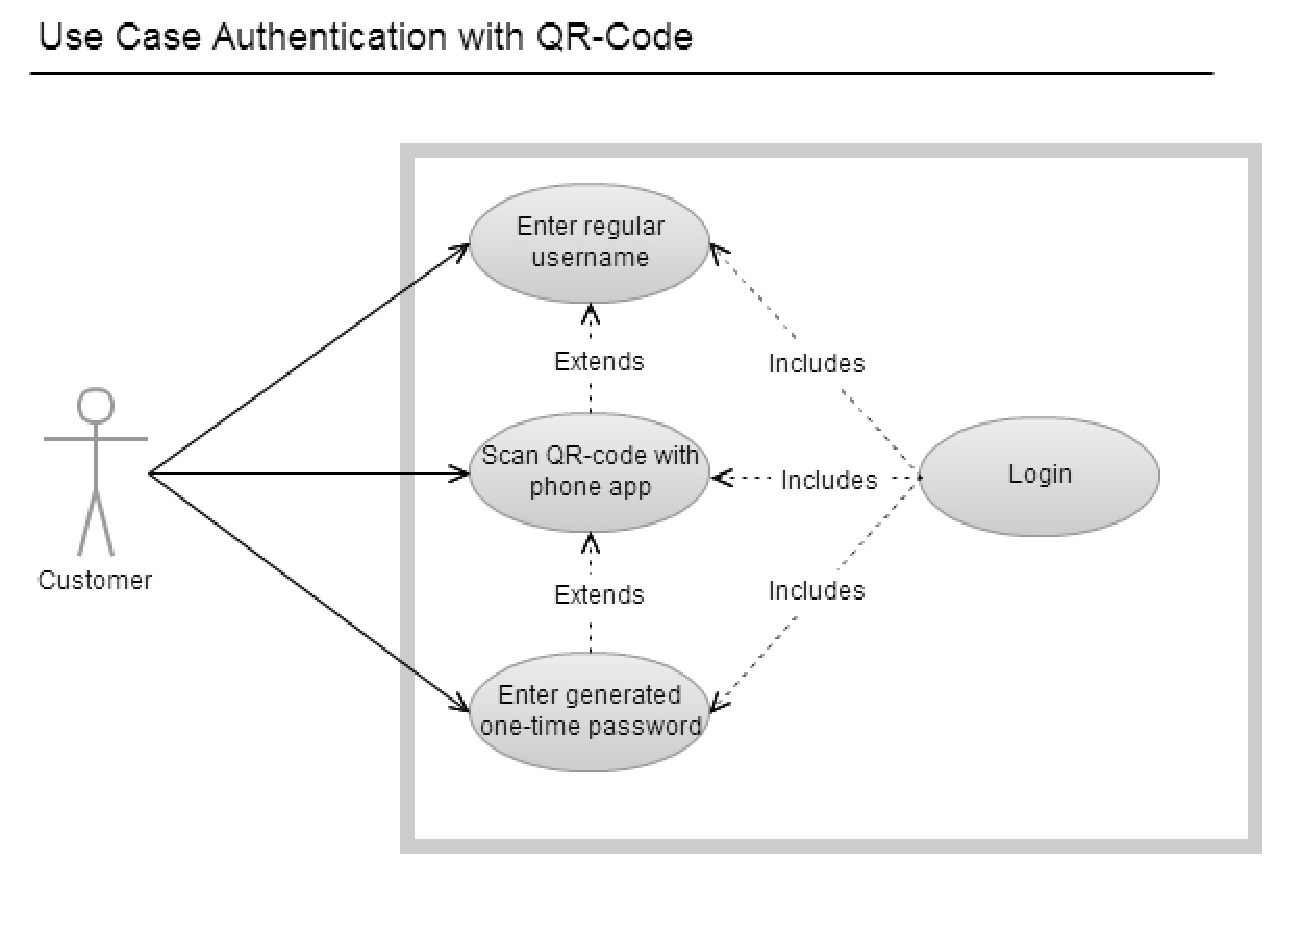
\includegraphics[width=\linewidth]{usecase.pdf}
\caption{To be able to login the user has to first type in the username, generate a one-time password using the application and then use the one-time password to log in.}
\label{fig:use-case}
\end{figure}


\begin{figure}[H]
%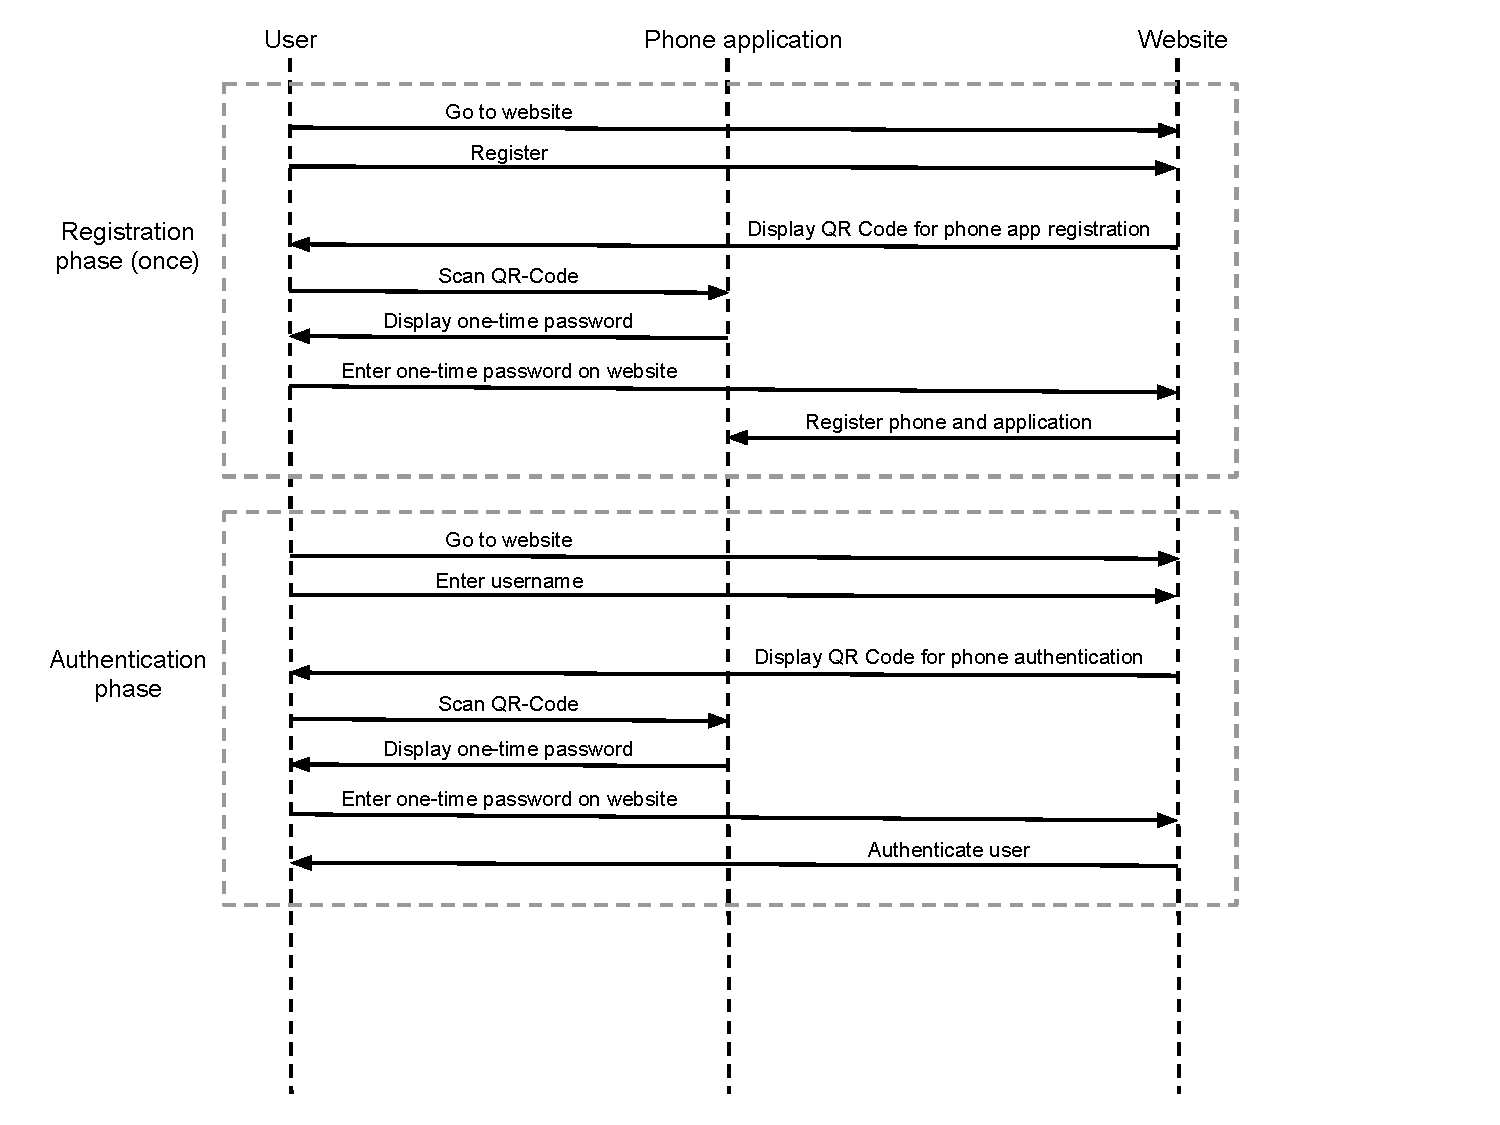
\includegraphics[width=\linewidth]{sequencediagram.pdf}
\caption{The sequence of actions to perform to authenticate with this method.}
\label{fig:sequence-diagram}
\end{figure}

\end{document}
